\documentclass{article}
\usepackage[francais]{babel}
\usepackage[UTF8]{inputenc}
\usepackage[T1]{fontenc}
\usepackage{graphicx}
\usepackage{fancyhdr}
\usepackage{eurosym}
\usepackage{color}
\usepackage{soul}

\pagestyle{fancyplain} \chead{}\lhead{\textit{Illogeeks}} \rhead{\emph{\textit{42 Days Later}}}



\begin{document}
\thispagestyle{empty}
\begin{center}
 \fontsize{42}{42}{\textbf{Cahier des charges \newline 42 Days Later}}
\end{center}

\begin{center}
 \fontsize{21}{21}{\textbf{- Team Illogeeks -}}
\end{center}

\vspace*{0.5cm}

\begin{center}
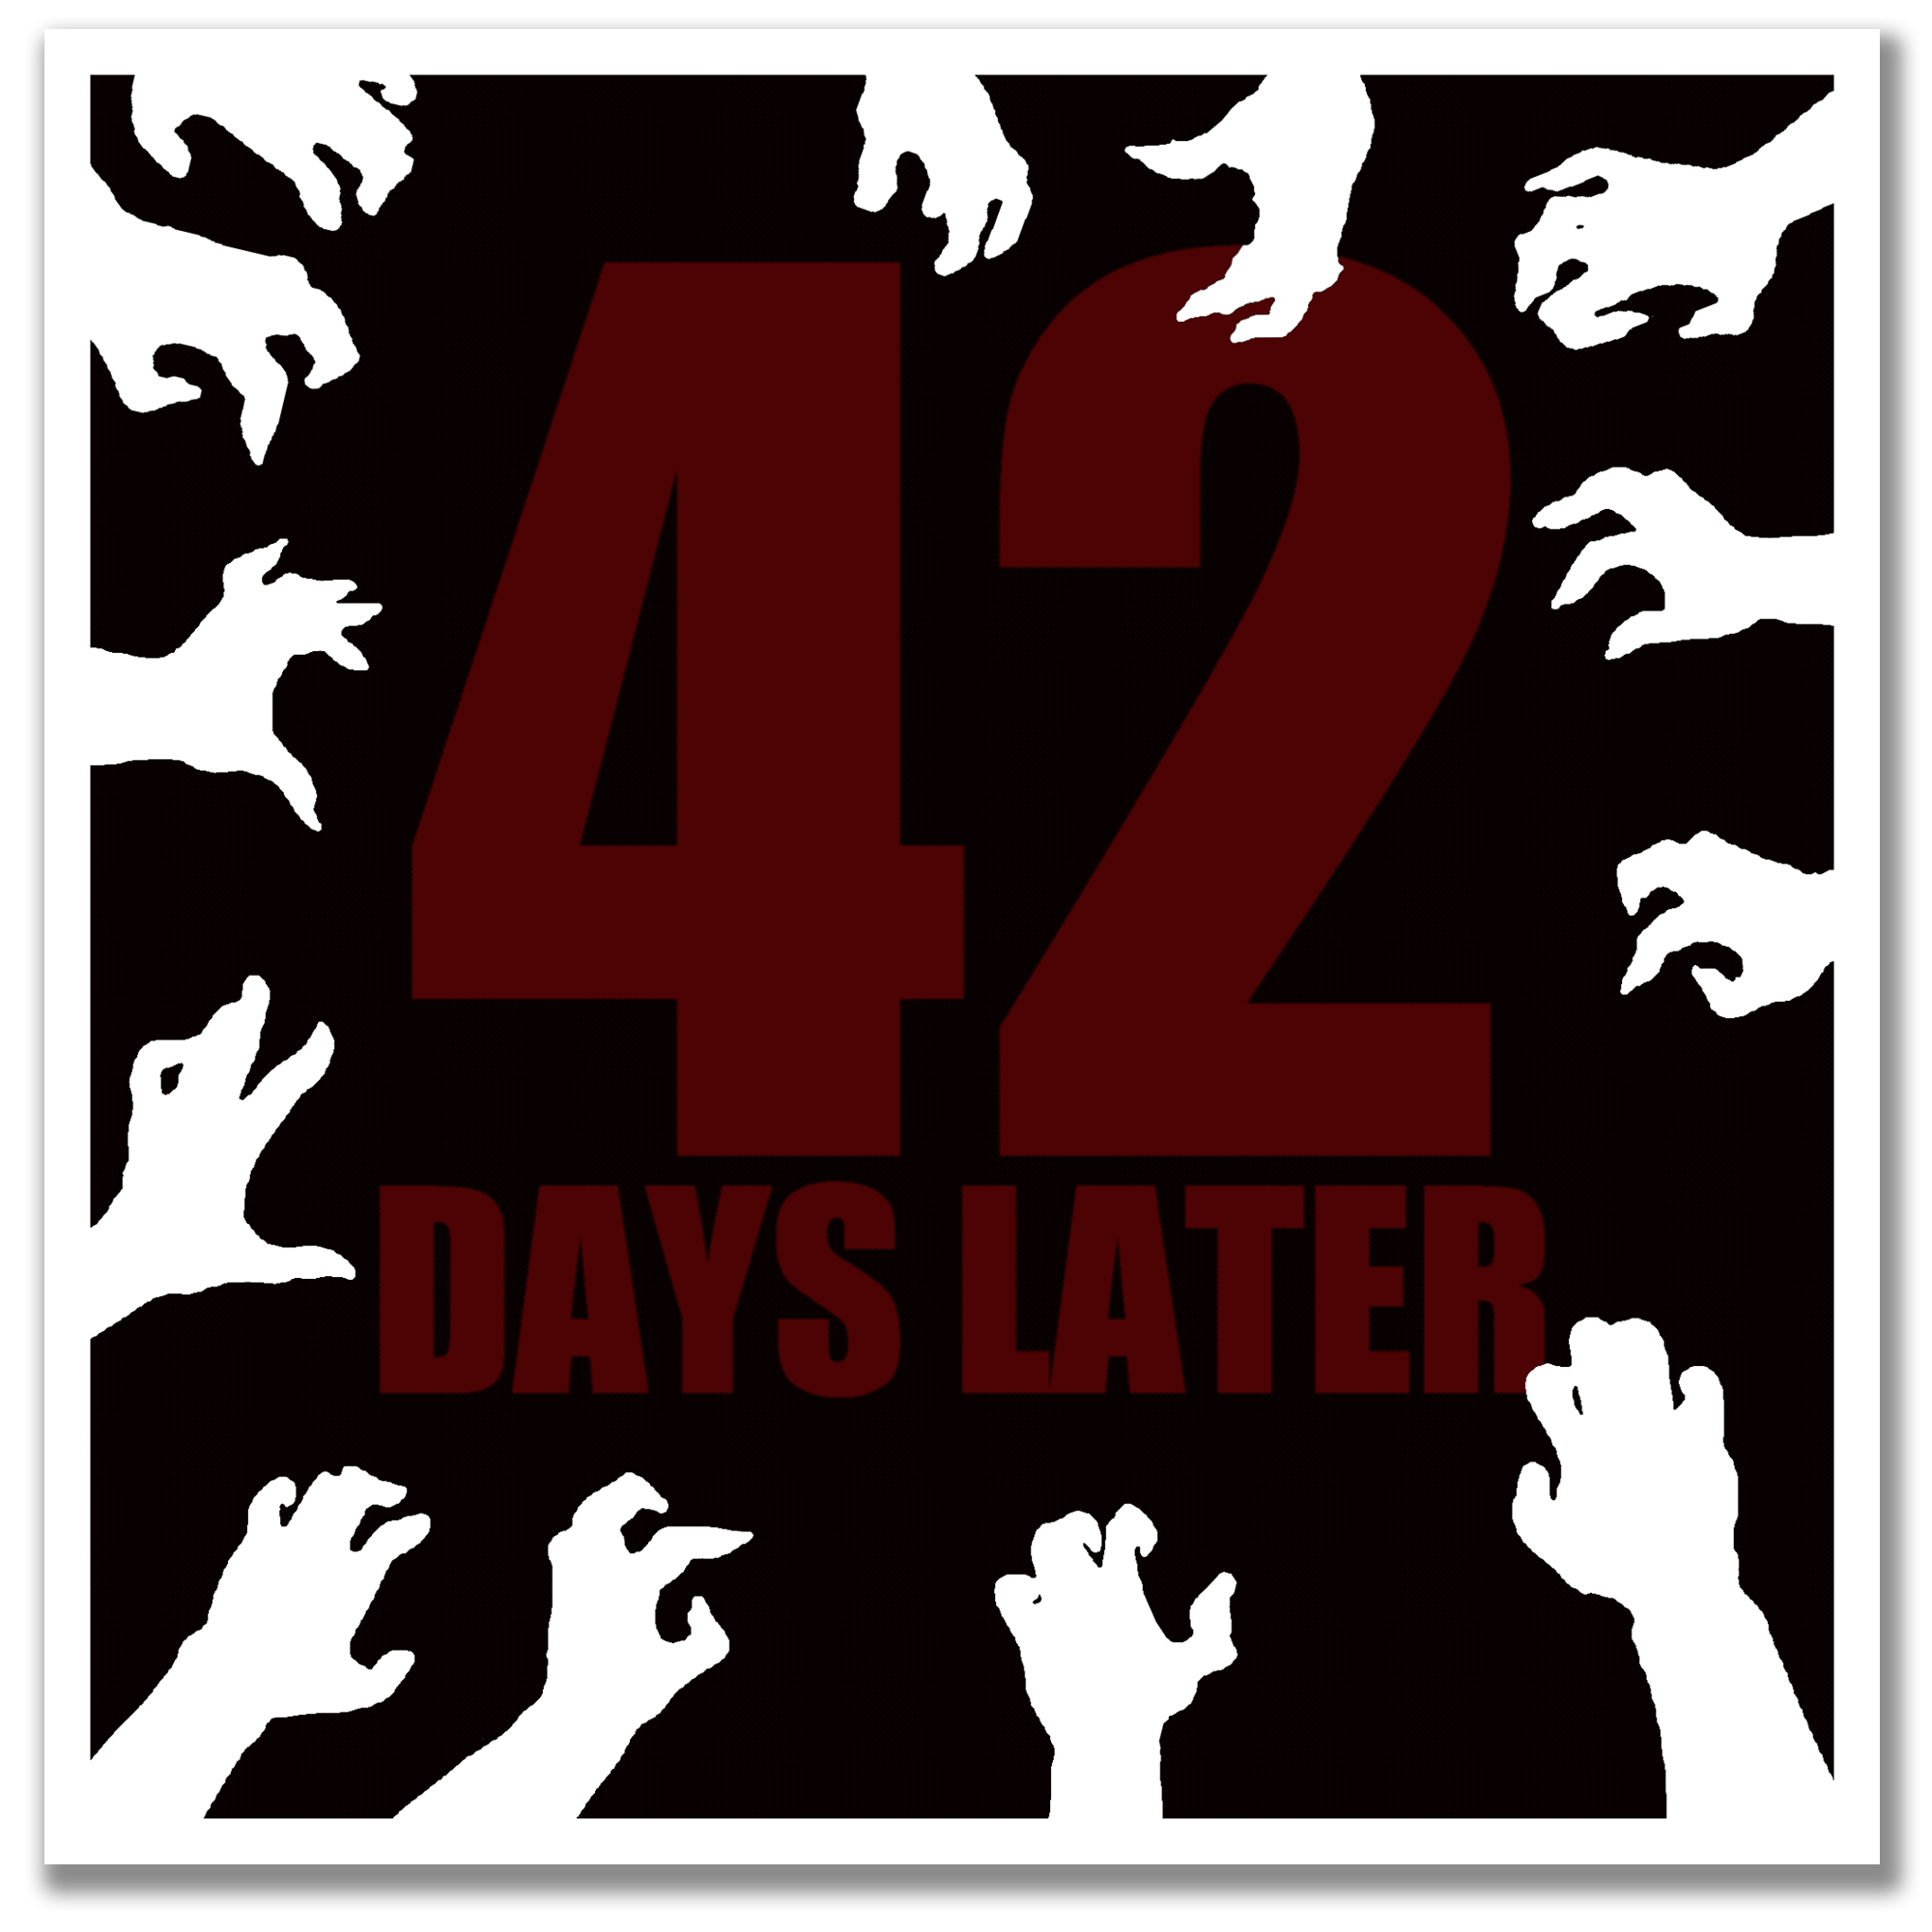
\includegraphics[scale=0.1]{Logo}
\end{center}

\vspace*{0.5cm}

\fontsize{14}{14}
\begin{center}
{SAHEL
\textcolor{red}{"The Architect"}
Roman - sahel\_r}
\end{center}
\begin{center}
MAGOT \textcolor{red}{"Amadeus"} Florian - magot\_f
\end{center}
\begin{center}
VERGER \textcolor{red}{"T3H BAGUETTE"} Hugo - verger\_h
\end{center}
\begin{center}
THUAULT \textcolor{red}{"Tapus"} Clément - thuaul\_c
\end{center}



\newpage
\thispagestyle{empty}
\tableofcontents



\newpage
\fontsize{12}{12}
\pagenumbering{arabic}
\section{Introduction}

\par
Nous, la Team Illogeeks, allons présenter notre projet informatique de première année à l'EPITA. Ce projet sera réalisé sur une durée d'environ 7 mois.
\newline


\subsection{Origines du groupe}

\par
Nous nous sommes rencontrés à l'EPITA cette année, et nous sommes rapidement entendus (Entre geeks, on s'entend toujours !). Tous les quatre en D1, nous avons facilement pu faire connaissance. En début d'année, nous nous sommes rencontrés puis avons rapidement décidé de partager l'expérience du projet d'informatique, étant donné que nous avions les mêmes intentions quant à sa nature.
\newline

\par
Même si nous ressemblons à des geeks qui passent leur temps sur les jeux vidéos, nous savons également quand il faut travailler ! Surtout quand le travail en question est coder un jeu vidéo.
\newline

\par
A l'unanimité, nous avons choisi de faire un Shoot them up en vue 2D isométrique, basé sur la survie à des hordes de zombies assoiffés de sang (On aime bien les idées originales). Ce type de jeu nous a attiré par le fait qu'il s'agisse d'un défi pour certains d'entre nous, par sa réalisation, et par le fait que le sujet même nous intéresse (Programmer un jeu, pas être des zombies !). C'est pour nous une occasion importante de réaliser ce jeu, et cela nous motive donc pour fournir un travail de qualité.
\newline

\par
Nous sommes donc impatients de nous mesurer à ce projet avec notre groupe récemment formé. Nous espérons que le travail d'équipe que nous aurons à fournir entrainera une collaboration durable.



\newpage
\subsection{Les \st{Geeks} Membres}
\subsubsection{ROMAN Sahel alias \textcolor{red}{"The Architect"}}

\par
Enchanté, je me présente, Roman Sahel, 18 ans, étudiant de première année à l’EPITA et efficace chef du projet 42 jours plus tard. L’informatique, c’est mon domaine : autant dire que j’y suis tombé dedans quand j’étais petit. Dès mon plus jeune âge, je me suis engagé dans le développement des programmes (que j’ai depuis conservé sur disquettes) aussi hétéroclites que complexes et alambiqués. C’est ainsi qu’à l’âge de 8 ans, j’ai notamment été mobilisé par la NASA pour concevoir le logiciel permettant de traiter les données du spectro-imageur de Mars Odyssey.
Malgré tout, ce projet est d’une certaine manière une première pour moi-même : en effet, je n’ai œuvré qu'en solitaire, si je puis dire : un travail en équipe est donc encore quelque chose d’inconnu mais qui ne m’effraie en aucun cas. De plus, mon équipe me paraît satisfaisante, et ce, même si à travers ma longue expérience professionnelle, j’ai rencontré des pontes de la programmation.
\newline

\par
Mais ce projet m’attire particulièrement car il nous pousse en avant vers la recherche, la création, l’imagination : créer quelque chose à partir de rien, un rêve trop souvent jugé inaccessible que moi et mes sujets allons tâcher d’accomplir avec grâce, beauté et perfection. N’ayons pas peur des mots : je suis plus que motivé, je suis prêt à me battre, sans relâche, jours et nuits, qu’il vente, qu’il pleuve ou qu’il fasse soleil, mes armes bien aiguisées à la main, je n’attends plus que les difficultés qui oseraient m’affronter.
\newline

\par
PS : mon pseudonyme se prononce avec l'accent américain étant donné qu’il m’a été donné par mes confrères anglophones de la NASA.
\newline

\subsubsection{MAGOT Florian alias \textcolor{red}{"Amadeus"}}

\par
Je vais vous épargner toutes les banalités du style “Grand Dieu \emph{(+1)} mais l’informatique est une véritable passion pour moi, j’y laisserais ma vie s’il le fallait”, ou autre “Diantre \emph{(+1)}, mais je suis en réelle symbiose avec le monde du jeu vidéo ! Je m’en doutais déjà, mais m’en rendre compte par moi-même est proprement renversant”. Oui, je l’avoue : \st{je me drogue}  je suis geek.
\newline

\par
Accessoirement, j’aime le cinéma aussi. Mais ça tout le monde s’en fout.
\newline

\par
Plus sérieusement, je pense que c’est une réelle chance d’avoir un projet comme celui-ci, à la fois ludique et formateur. Je n’ai jamais vraiment eu le courage (et la folie) pour me lancer dans une réalisation en solitaire, ce sera donc une grande première pour ma part. Mais c’est avec joie que je me plonge la tête la première dans le monde merveilleux (et tout plein de poneys) du C\#.
\newline

\par
Nonobstant \emph{(+1)} mes faibles connaissances en programmation, je compte bien apporter une réelle valeur ajoutée au projet grâce à mes talents un peu plus artistiques (et à ma motivation !). De toute façon on sera les meilleurs, je me fais pas de soucis là-dessus.
\newline

\par
Parce qu’on a beau dire, dégommer du zombie ça roxx.
\newline

\subsubsection{VERGER Hugo alias \textcolor{red}{"T3H BAGUETTE"}}

\par
Salut ! Moi c'est Baguette et je suis un Geek niveau 42. Et toi à quoi tu joues ?
\newline

\par
Pour aller au plus simple et se faire une idée de ma supériorité, je pense qu'on pourrait me qualifier de geek / gamer / nerd / nolife / otaque / cinéphile / quelqu'un de ponctuel (Rayez la mention inutile).
\newline

\par
En résumé, côté informatique, j'ai touché à quasiment tout autant au niveau hardware que software (photoshop, musique, création de vidéos...), et comme tout bon geek qui se respecte, quand quelque chose chose attire ma curiosité, je me passionne vite et j'apprends en autodidacte.
\newline


\par

\par
J'ai ajouté la programmation à ma liste d'intérêts depuis 1 an histoire de parfaire le cliché.  Je me suis habitué au Java donc le passage au C\# s'est fait sans soucis. 
\newline

\par
Les zombies c'est aussi une de mes grandes passions depuis longtemps sur tous les supports : Films, Séries, Animes, Romans, BD, Mangas, Jeux Vidéos...  Il n'existe rien à ma connaissance sur les zombies que je n'aurais pas consulter, alors créer un jeu de shoot de zombie c'est vraiment quelque chose qui me délecte !
\newline

\fontsize{9}{9}
\par
\small Bon, entre nous, les gars avec moi sont un peu des bras cassés mais ça me va car sans handicap il faudrait me noter sur 40 (J’ai oublié d'ajouter la modestie à la liste de mes qualités).
\newline

\par

\fontsize{12}{12}
\par
\normalsize Tout ça pour dire que notre jeu va être le meilleur jeu de tous les temps, préparez vous, Illogeeks arrivent et on va retourner la baraque !
\newline




\newpage
\subsubsection{THUAULT Clément alias \textcolor{red}{"Tapus"}}

\par
J'ai toujours été un gros joueur de jeux vidéos, un peu geek, voire même à certains moments carrément nolife, à tel point que je me suis un jour dit : "Mais pourquoi pas, un jour, en créer un ?". Étant souvent seul chez moi, mon ordinateur est un peu mon meilleur ami ! C'est pourquoi je me suis en quelque sorte engagé dans cette voie qu'est l'informatique. Car oui, c'est une véritable passion pour moi, j'y laisserais ma vie (sociale !) s'il le fallait.
\newline

\par
J'ai commencé à programmer au lycée, des petits jeux de plateau en 2D, et j'attendais impatiemment le moment ou je pourrais coder un vrai jeu vidéo, digne de ce nom (Parce que le Démineur, ça va 5 minutes...) Je n'avais à l'époque évidemment pas le temps de m'engager dans une telle réalisation. Maintenant que je dois en faire un, je serai évidemment plus motivé que jamais !
\newline

\par
C'est pourquoi je pense donc apporter ma touche personnelle au projet que nous avons à réaliser. Étant un peu perfectionniste et touche-à-tout, je prends ce projet à cœur. J'apprécie le fait de travailler en groupe, car c'est une très bonne expérience et cela reflète déjà le travail en entreprise, à plusieurs.
\newline



\newpage
\subsection{Le projet}

\par
Le projet que nous allons présenter dans ce cahier des charges est donc un jeu en vue 2D isométrique, c'est-à-dire une vue de dessus inclinée à 45\textdegree. Ce jeu sera donc de type survie, shooter ; le but principal du projet est de faire un mode par vagues, c'est-à-dire que les ennemis, les zombies, apparaîtront par vagues, et le but sera donc de les éliminer.
\newline

\par
C'est donc un projet en C\# qui a été choisi, avec la surcouche XNA. En effet, il nous semblait plus raisonnable d'utiliser un langage impératif auquel la plupart d'entre nous étaient habitués, avec l'utilisation d'XNA, bibliothèque très complète qui nous semble être la plus adaptée possible pour un premier jeu en 2D isométrique. Nous sommes impatients de pouvoir tester les nombreuses possibilités de ce langage et de cette bibliothèque. Nous n'aurions certainement pas eu le courage de commencer à programmer avec des langages ou des bibliothèques bien plus complexes et bien moins efficaces, c'est pourquoi le choix fut très rapide.
\newline

\par
Nous nous sommes en effet directement inspirés d'un jeu s'appelant \emph{Zombie Shooter} qui reprenait ce même système. Mais, qu'est-ce qu'un shooter en vue isométrique ? Basiquement, le système est très simple : le joueur contrôle un personnage, ses déplacements, la visée de son arme, et doit donc éliminer tous les ennemis à l'instar d'un FPS (First Person Shooter = Vue à la Première Personne) classique. La seule différence est que cette vue est donc placée non pas dans la vision du personnage, mais au dessus de lui, avec un plan incliné. Nous voulions en effet développer les mouvements et la liberté d'action que la 2D isométrique permet, contrairement à la 2D. En revanche, l'utilisation de la 3D aurait gaspillé les ressources de la machine, en plus d'avoir un rendu graphique moins soigné, sans compter le fait que ce passage à la 3D n'apporterait rien à la jouabilité actuelle.
\newline

\par
Soit dit en passant, le titre du jeu est directement inspiré du film : "28 jours plus tard". Sauf que maintenant, c'est 42 jours. Et non pas 28.
\newline

\par
Ce qui caractérise ce type de jeu est donc le fait qu'il n'y ait pas de réelle complexité dans la jouabilité. Nous essaierons de faire le jeu le plus simple possible, tout en ajoutant un certain nombre de bonus et d'évènements qui rendent le jeu agréable à jouer, tout en restant simple. Le but final est donc de survivre à toutes les vagues de zombies... En les exterminant. Enfin, la difficulté n'en sera pas pour autant réduite, bien au contraire. De nombreuses modifications seront possibles pour régler la difficulté ainsi que le choix de la carte.
\newline

\par
Développons maintenant les différentes parties du projet, concernant sa réalisation.
\newline



\newpage
\section{Découpage du projet}
\subsection{Les commandes et le gameplay}
\subsubsection{Les commandes}

\par
Tout d'abord, les commandes sont très basiques, on a donc :
\newline

\par
\textbf{Les déplacements :} Le personnage se déplacera grâce au clavier, tout simplement, avec différents réglages dans les options selon le type de clavier (AZERTY, QWERTY, ou bien tout simplement les flèches directionnelles).
\newline

\par
\textbf{Les tirs :} Nous essaierons d'attribuer au personnage un certain arsenal, afin de varier les armes, mais leur utilisation sera toujours la même. On a donc une visée grâce au curseur de la souris, à 360\textdegree . Le personnage s'orientera directement vers le curseur (Oui, souvent on regarde là ou on tire, c'est plus efficace.) et les tirs se feront grâce au clic gauche. Notons que la portée de l'arme sera fixe, c'est à dire que le projectile ne s'arrêtera pas à la position du curseur, mais bien après une certaine distance, déterminée au préalable.
\newline

\par
\textbf{Le rechargement :} Comme dans beaucoup de jeux, le rechargement se fera avec la touche R, ou bien une touche plus proche des flèches directionnelles.
\newline

\par
Comme vous pouvez le constater, il y a donc un gameplay qui pourrait sembler trop basique ; mais ce gameplay est parfaitement intégré dans un jeu nerveux qui permet donc de se défouler et de donner une bonne dose de fun.
\newline

\subsubsection{Le gameplay}

\par
Concernant les mécaniques du jeu, le gameplay, nous souhaitons principalement créer un mode Survie.
\newline

\par
\textbf{Mode Survie :} Il y aura donc plusieurs manches dans le mode Survie, plusieurs vagues de zombies. Au fur et à mesure, ces vagues sont plus longues, sont plus difficiles à franchir, et font apparaître de plus en plus de zombies.
\newline

\par
Ces zombies apparaîtront aléatoirement, dans certaines zones libres (c'est-à-dire des zones où il n'y aura pas de collision sur la carte), hors du champ de vision de la caméra. En effet, les ennemis ne doivent pas miraculeusement apparaître devant notre personnage !
\newline



\newpage
\par
\textbf{Concernant les tirs :} Nous ferons un système de tir en continu (Sans avoir à cliquer n fois sur la souris pour tirer n projectiles) dans la limite de la fréquence de tir. Le personnage aura également besoin de recharger tous les n tirs --- son chargeur n'étant pas sans fond --- obligatoire lorsque le chargeur en question est vide.
\newline

\par
Enfin, il est également probable qu'il soit intégré une chance de "Coup Critique" ou de "Headshot" en fonction de la portée, de l'aléatoire, ou du temps qu'il fait en Suède.
\newline

\par
\textbf{Santé :} Le personnage, tout comme les zombies, n'est pas immortel. C'est pourquoi il aura donc une jauge de vie, qui sera décrémentée selon le nombre de dégats que lui aura causé le zombie, lors d'une attaque. De même, les zombies subissent également des dégâts, traités de la même façon.
\newline

\par
Le jeu se termine lorsque le héros est mort, \textit{Game Over}, ou bien lorsque toutes les manches ont été passées, et que vous avez tout exterminé sur votre passage, \textit{Félicitations !}, ou encore parce que.. vous avez quitté le jeu.. \textit{RAGEQUIT}.
\newline

\subsection{Le moteur physique et l'IA}

\par
Concernant le moteur physique, nous l'utiliserons pour faciliter les collisions avec le décor, et les autres entités du jeu (comme le personnage, les zombies). Cela nous permettra également de régler des attributs physiques éventuels, comme la charge à travers un groupe de zombies, réduisant alors la vitesse du personnage.
\newline

\par
De nombreuses possibilités sont donc possibles avec le moteur physique que nous utiliserons, associé à XNA (Il s'agit de Farseer Physics Engine). Nous pensons également ajouter, grâce à ce moteur physique, des particules, comme la pluie, le sang, la brume... afin de donner un aspect plus réaliste et une ambiance plus immersive.
\newline

\par
\textbf{IA :} Enfin, il faut bien que les zombies sachent retrouver notre héros, afin de le poursuivre inlassablement en criant : \textit{"CERVEAU !"}. C'est pourquoi l'IA tâchera de trouver la position du joueur, et s'y orientera, en évitant les obstacles grâce à l'utilisation du pathfinding. Lorsque le joueur sera à portée d'attaque du zombie, ce dernier pourra alors l'attaquer.
\newline



\newpage
\subsection{Les graphismes}

\par
Dans un jeu, il faut un minimum de (beaux) graphismes pour le faire fonctionner correctement. Nous allons voir lesquels sont nécessaires à notre projet.
\newline

\subsubsection{Les sprites, les animations de jeu}

\par
Tout d'abord, le jeu fonctionnera avec des \textit{sprites}, qui sont des éléments graphiques se déplaçant sur l'écran de jeu.
\newline

\par
C'est pourquoi nous utiliserons, dans le cadre de la 2D isométrique, \textbf{8 orientations} pour les personnages et les zombies. En effet, cette vue nous oblige à être plus précis quant à cette orientation du personnage. Le personnage regarde-t-il vers le Nord, ou vers le Sud-Est ?
\newline

\par
Les personnages auront donc une animation de course, et seront donc animés, grâce à une succession de sprites. Le sprite choisi sera donc en fonction de l'orientation donnée par la position du curseur.
\newline

\par
Enfin, la \textbf{carte} sera aussi partie intégrante des graphismes, et devra gérer les collisions. Nous prévoyons d'en ajouter pour allonger la durée de vie du jeu.
\newline

\subsubsection{Les médias}

\par
Dans cette partie, nous allons détailler les médias dont nous aurons besoin pour notre projet, mais qui ne seront pas partie intégrante du jeu en soi. Cela inclut donc :
\newline

\par
\textbf{Une introduction} afin de présenter le nom du projet et du groupe, ainsi \textbf{qu'une courte vidéo} présentant le jeu lui-même.
\newline

\par
Nous aurons également besoin des éléments du menu, dont nous allons parler plus en détail en partie 2.6.1.
\newline

\par
Par la suite, il sera alors possible de regrouper tous ces médias dans une section du Site web. Nous pensons ajouter à cela des élements tels que des fonds d'écran, des icônes, des logos et enfin des bannières.
\newline



\newpage
\subsection{Le réseau}

\par
Vous n'êtes pas seul dans ce monde rempli de zombies ! Le réseau est ici un passage obligatoire pour le mode multijoueur, car les commandes (Au clavier et à la souris) ne sont pas partageables sur un seul écran.
\newline

\par
C'est pourquoi il sera donc nécessaire d'établir un système de LAN par connexion directe, c'est-à-dire par IP.
\newline

\par
Cela entrainera donc l'apparition d'un autre personnage dans le jeu. Les joueurs seront donc amenés à faire face à des vagues de zombies de plus en plus importantes.
Dans le cas d'une partie à 2 joueurs, on peut donc estimer que la vague sera, par exemple, 2 fois plus difficile, avec 2 fois plus d'ennemis.
\newline

\par
D'autre part, il faudra également que l'apparition des zombies ne se fasse pas dans le champ de vision des joueurs.
\newline

\par
Le jeu en multijoueur, en réseau semble intéressant mais complexe à mettre en place. Cela permet en effet d'ajouter une autre dimension au jeu, en coopératif.
\newline

\subsection{Les sons}

\par
Que serait un jeu de zombies.. sans son ? L'ambiance est un facteur important dans un jeu de ce type. C'est pourquoi nous aurons besoin de plusieurs sons :
\newline

\par
\textbf{Ambiance sonore :} Il faudra une ambiance sonore tout au long du jeu, afin de maintenir une certaine tension sur le joueur. Le but est de rendre le jeu plus immersif grâce aux sons.
\newline

\par
\textbf{Tirs :} Bien entendu, les tirs de l'arme seront enregistrés et modifiés selon l'arme utilisée (On n'aura évidemment pas le même son pour un pistolet que pour une tronconneuse..)
\newline

\par
\textbf{Zombies :} Ensuite, il y aura des sons pour les cris et les attaques des zombies, toujours dans le but de rendre le jeu plus réaliste. 
\newline

\par
\textbf{Personnage :} Qui a dit que le personnage était muet ? Le personnage fera effectivement des commentaires vocaux de façon aléatoire.
\newline

\subsection{L'interface}

\subsubsection{Le menu principal}

\par
Le menu principal est un élément essentiel car il est le premier écran après la vidéo d'introduction. Il sera donc composé de plusieurs boutons :
\newline

\par
\textbf{Solo :} Accès au jeu solo, le mode survie. On peut alors sélectionner la carte et la difficulté du jeu.
\newline

\par
\textbf{Multijoueur Réseau :} Ce mode donnera accès à une connexion directe par IP, créant alors une instance de jeu en multijoueur.
\newline

\par
\textbf{Options :} Il sera possible de voir les commandes du jeu, et il sera également possible de changer la résolution, et de mettre le jeu en plein écran. Enfin, il sera possible de changer la langue du jeu.
\newline

\par
\textbf{Quitter :} Cela semble évident, il est également possible de quitter le jeu. 
\newline

\subsubsection{En jeu}

\par
En jeu, il y aura deux types d'interface :
\newline

\par
\textbf{Le menu pause} accessible en appuyant sur Echap, à partir duquel il sera possible de reprendre la partie, recommencer la partie ou de quitter le jeu.
\newline

\par
\textbf{L'interface du jeu} qui contiendra donc la jauge de vie du personnage, le nombre de munitions restantes, la vague actuelle et le nombre d'ennemis restants.
\newline



\newpage
\subsection{Site Web}

\par
Le site web va être notre carnet de route tout au long du projet. Un historique de nos projets, de nos versions de jeu, de nos divers rapports sera inclus. Nous y incluerons également les problèmes auxquels nous avons été confrontés, ainsi que les solutions que nous avons pu y apporter.
\newline

\par
Ces rapports et exécutables seront également disponibles dans une section de téléchargement.
\newline

\par
De plus, nous ajouterons une page de présentation du groupe, des membres, et également du projet.
\newline

\par
Enfin, le site contiendra également une section "médias" contenant des fonds d'écran, logos, et d'autres ressources dont nous avons eu besoin pour notre projet.
\newline

\par
Il est donc important de mettre ce site à jour, pour renseigner les visiteurs sur l'avancement du projet.
\newline



\newpage
\section{Répartition des tâches}
\subsection{Répartition entre les membres du groupe}

\par
Même si une répartition des tâches est nécessaire, nous souhaitons faire en sorte que chacun des membres du groupe puisse programmer, participer à la réalisation de sprites ou encore à l'implémentation du moteur physique. Il nous semble normal de se regrouper à plusieurs dans une tâche pour mieux se répartir différents domaines de travail.
\newline

\par
Il semble plus judicieux de travailler en groupe, en commun sur certains aspects, plutôt que de faire notre travail séparément sans faire un lien dans le groupe.
\newline

\par
Légende : $\times$ : Doit effectuer cette tâche

\begin{center}
\begin{tabular}{|c|c|c|c|c|}
\hline
 & Roman & Florian & Hugo & Clément \\
\hline
Commandes et gameplay & $\times$ & & $\times$ & \\
\hline
Moteur physique et IA & $\times$ & & $\times$ & \\
\hline
Graphismes & $\times$ & $\times$ & & \\
\hline
Réseau & & & & $\times$ \\
\hline
Sons & $\times$ & $\times$ & $\times$ & $\times$ \\
\hline
Interface & & $\times$ & & \\
\hline
Site Web & & & & $\times$ \\
\hline
\end{tabular}
\end{center}

\begin{center}
\bf{Fig. 1 : Répartition initiale entre les membres du groupe}
\end{center}



\newpage
\subsection{Avancement}

\par
L'avancement est noté dans le tableau avec des pourcentages.
\newline

\subsubsection{1ère soutenance}

\begin{center}
\begin{tabular}{|c|c|c|c|c|}
\hline
 & Roman & Florian & Hugo & Clément \\
\hline
Commandes et gameplay & 30\% & & 30\% & \\
\hline
Moteur physique et IA & 25\% & & 25\%  & \\
\hline
Graphismes & 20\% & 20\% & & \\
\hline
Réseau & & & & 10\% \\
\hline
Sons & 10\% & 10\% & 10\% & 10\% \\
\hline
Interface & & 20\% & & \\
\hline
Site Web & & & & 10\% \\
\hline
\end{tabular}
\end{center}

\begin{center}
\bf{Fig. 2 : Répartition à la 1ère soutenance}
\end{center}

\subsubsection{2ème soutenance}

\begin{center}
\begin{tabular}{|c|c|c|c|c|}
\hline
 & Roman & Florian & Hugo & Clément \\
\hline
Commandes et gameplay & 65\% & & 65\% & \\
\hline
Moteur physique et IA & 50\% & & 50\% & \\
\hline
Graphismes & 45\% & 45\% & & \\
\hline
Réseau & & & & 45\% \\
\hline
Sons & 40\% & 40\% & 40\% & 40\% \\
\hline
Interface & & 50\% & & \\
\hline
Site Web & & & & 30\% \\
\hline
\end{tabular}
\end{center}

\begin{center}
\bf{Fig. 3 : Répartition à la 2ème soutenance}
\end{center}



\newpage
\subsubsection{3ème soutenance}

\begin{center}
\begin{tabular}{|c|c|c|c|c|}
\hline
 & Roman & Florian & Hugo & Clément \\
\hline
Commandes et gameplay & 90\% & & 90\% & \\
\hline
Moteur physique et IA & 75\% & & 75\% & \\
\hline
Graphismes & 70\% & 70\% & & \\
\hline
Réseau & & & & 65\% \\
\hline
Sons & 70\% & 70\% & 70\% & 70\% \\
\hline
Interface & & 80\% & & \\
\hline
Site Web & & & & 75\% \\
\hline
\end{tabular}
\end{center}

\begin{center}
\bf{Fig. 4 : Répartition à la 3ème soutenance}
\end{center}

\subsubsection{4ème soutenance - Soutenance Finale}

\begin{center}
\begin{tabular}{|c|c|c|c|c|}
\hline
 & Roman & Florian & Hugo & Clément \\
\hline
Commandes et gameplay & 100\% & & 100\% & \\
\hline
Moteur physique et IA & 100\% & & 100\% & \\
\hline
Graphismes & 100\% & 100\% & & \\
\hline
Réseau & & & & 100\% \\
\hline
Sons & 100\% & 100\% & 100\% & 100\% \\
\hline
Interface & & 100\% & & \\
\hline
Site Web & & & & 100\% \\
\hline
\end{tabular}
\end{center}

\begin{center}
\bf{Fig. 5 : Répartition à la soutenance finale (Complet)}
\end{center}



\newpage
\section{Coût de production}

\par
Voici le coût de production de notre projet. Le matériel, les logiciels, tout est pris en compte, mais nous avons un budget très serré ! C'est pourquoi nous serons certainement un des groupes les plus économes de cette promotion !
\newline

\begin{center}
\begin{tabular}{|c|c|}
\hline
Année à l'EPITA \(\times\) 4 & 22800 \euro \\
\hline
Ordinateur \(\times\) 4 & 4000 \euro \\
\hline
Adobe Master Collection CS5 & 2500 \euro \\
\hline
Cargaisons de Kinder Bueno, de Pépitos, et de Redbull  & 1337 \euro \\
\hline
42 Pizzas & 420 \euro \\
\hline
T-Shirts & 80 \euro \\
\hline
DVD, Jaquette, Manuel & 20 \euro \\
\hline
Nom de domaine & 10 \euro \\
\hline
Esclaves & 3,1415926535 \euro \\
\hline
\st{Pot-de-vin} Cadeau pour Krisboul & 666 \euro \\
\hline
Fête la veille de la soutenance finale & $10^{51}$ \euro \\
\hline
Total & \(\infty\)  \\
\hline
\end{tabular}
\end{center}

\begin{center}
\bf{Fig. 6 : Coût de production (C'est un peu cher, non ?)}
\end{center}

\vspace*{2cm}

\begin{center}
\includegraphics[scale=0.5]{Dollars}
\end{center}



\newpage
\section{Conclusion}

\par
Notre projet est donc basé sur un Shoot them up en 2D isométrique et représente un grand défi pour nous. C'est pourquoi nous sommes motivés et prêts à réaliser ce jeu complet. Avec un mode solo et multijoueur, le jeu semble prometteur et nous espérons mener à bien ce projet. Le travail personnel et collectif que nous avons a fournir tend à enrichir notre propre expérience. 

\vspace*{6cm}

\par
\begin{center}
\textcolor{red}{\emph{"Ni nostalgeeks, ni amnégeeks, ni paraplégeeks, nous sommes les Illogeeks !"}}
\end{center}



\end{document}
























